\lecture{8}{lun 01 mag 2023 17:14}{Linearizzazione}
	\lablsection{Linearizzazione}
	Consideriamo piccoli spostamenti nell'interno dei punti di equilibrio. Considero un'approssimazione lineare nell' intorno del punto
	\begin{equation*}
		\begin{cases}
			\dot{x}(t) = f(x(t),u(t))\\
			y = g(x(t),u(t))
		\end{cases}
	\end{equation*}
	Considero $ u=\overline{u} $ $ \forall t\geq0 $ e calcolo $ (\overline{x},\overline{y}) $, con $ \overline{x} $ stato di equilibrio e $ \overline{y} $ uscita di equilibrio. Li ottengo come:
	\begin{equation*}
		\begin{cases}
			f(\overline{x},\overline{y}) = 0\\
			\overline{y} = g(\overline{x},\overline{y})
		\end{cases}
	\end{equation*}
	Considero piccoli spostamenti intorno a $\overline{x},\overline{u},\overline{y}$:
	\[\text{per } t=0 \quad x_0 =\overline{x}+\delta x_0\]
	Analogamente ho $ \forall t\geq0 $:
	\begin{align}
		u(t)&=\overline{u}+\delta u(t)\\
		x(t)&=\overline{x}+\delta x(t)\\
		y(t)&=\overline{y}+\delta y(t)\\
	\end{align}
	Le equazioni del sistema si scrivono come:
	\begin{equation*}
		\begin{cases}
			\dot{x}(t) = f(\overline{x}+\delta x(t),\overline{u}+\delta u(t))\\
			y(t) = g(\overline{x}+\delta x(t),\overline{u}+\delta u(t))
		\end{cases}
	\end{equation*}
	Sfrutto la serie di \person{Taylor} arrestata ai termini di primo grado e trovo:
	\begin{align}
		\delta\dot{x}(t) =\overbrace{ \pdev{f}{x}}^\text{\textcolor{red}{A}}|_{\overline{x},\overline{u}}\,\,\delta x(t)+\overbrace{\pdev{f}{u}}^\text{\textcolor{red}{B}}|_{\overline{x},\overline{u}}\,\,\delta u\\
		\delta y(t) =\overbrace{\pdev{g}{x}}^\text{\textcolor{red}{C}}|_{\overline{x},\overline{u}}\,\,\delta x(t) +\overbrace{\pdev{g}{u}}^\text{\textcolor{red}{D}}|_{\overline{x},\overline{u}}\,\,\delta u
	\end{align}
	Il sistema linearizzato:
	\begin{equation*}
		\begin{cases}
			\delta\dot{x}(t) = A\delta x(t) + B \delta u(t)\\
			\delta y (t) = C \delta x(t) + D\delta u(t)
		\end{cases}
	\end{equation*}
	\lablsubsection{Stabilità degli stati di equilibrio di un sistema non lineare}
	Studiare la stabilità degli stati di equilibrio considerando i corrispondenti sistemi linearizzati
	\subsubsection{Teorema di stabilità dei punti di equilibrio di sistemi non lineari}
	Sistema non Lineare:
	\begin{equation*}
		\begin{aligned}
			& \dot{x}(t)=f(x(t), \mu(t)) \\
			& y(t)=f(x(t), \mu(t))
		\end{aligned}
	\end{equation*}
	E si consideri l'equazione di stato e si supponga di linearizzare nell'intorno di $\overline{x}$ dato $\overline{u}$.\\
	La matrice della dinamica sarà:
	\begin{equation*}
		A=\left.\frac{\partial f}{\partial x}\right|_{\bar{x}, \bar{u}}
	\end{equation*}
	Allora vale che:
	\begin{itemize}
		\item Se la matrice A ha autovalori a parte reale strettamente negativa $\to$ A.S.
		\item Se la matrice A ha almeno un autovalore a parte reale positiva $\to$ Instabile
	\end{itemize}
	\nota{Il primo punto del teorema è condizione sufficiente ma non necessaria e se A non ha autovalori a parte reale positiva ma ha parte reale nulla, non posso trarre conclusioni.}
	\lablsubsection{Proprietà dei sistemi A.S.}
	\begin{itemize}
		\item Un sistema A.S. presenta per ingressi nulli movimenti che tendono a zero per $ t \to \infty $.
		\item Lo stesso vale nel caso di ingressi di durata limitata.
		\item Nel caso di un impulso, la risposta dello stato tende a zero.
	\end{itemize}
	\lablsubsection{Sistemi nel dominio della frequenza}
	Voglio calcolare la risposta di un sistema LTI soggetto a certi ingressi. Ci sono due modi:
	\begin{enumerate}
		\item Nel dominio del tempo: risolvo le equazioni differenziali forzate dagli ingressi. Poi dalle trasformate di uscita valuto $y(t)$
		\item Nel dominio della frequenza: A $u(t)$ corrisponde $U(s)$, chiamata trasformata di \person{Laplace} di $ u(t) $. Faccio la stessa trasformazione con lo stato e ottengo equazioni in $ X(s) $,
		trasformata di \person{Laplace} dello stato. Dato $ U(s) $ e le equazioni algebriche in $ X(s) $, ricavo $ Y(s) $ e antitrasformo per ottenere $ y(t) $.
	\end{enumerate}
	\begin{figure}[H]
		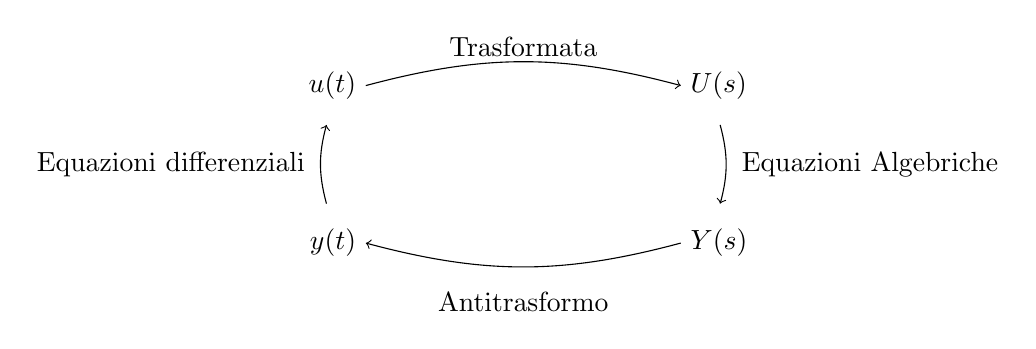
\begin{tikzpicture}
			\centering
			\draw[->] (-2,-1) node[left]{$ u(t) $} to[bend left = 15] (2,-1) node[right]{$ U(s) $};
			\draw (0,-0.75) node[above]{Trasformata};
			\draw[->] (2.5,-1.5) to[bend left = 15] (2.5, -2.5);
			\draw (2.65,-2) node[right]{Equazioni Algebriche};
			\draw[<-] (-2,-3) node[left]{$ y(t) $} to[bend right = 15] (2,-3) node[right]{$ Y(s) $};
			\draw (0,-3.5) node[below]{Antitrasformo}; 
			\draw[<-] (-2.5,-1.5) to[bend right = 15] (-2.5, -2.5);
			\draw (-2.65,-2) node[left]{Equazioni differenziali};
		\end{tikzpicture}
	\end{figure}
	\lablsubsection{Trasformata di Laplace}
	Sia $ f(t) $ funzione del tempo $ t\geq 0 $. Chiamo $ s $ la variabile complessa di \person{Laplace}. Si dice trasformata di \person{Laplace} di $ f(t) $ la funzione
	\begin{equation*}
		F(s) = \int_{0}^{\infty} f(t) e^{st}dt
	\end{equation*}
	La trasformata si indica anche come: 
	\begin{equation*}
		\mathcal{L}[f(t)]
	\end{equation*}
	\lablsubsection{Segnali Canonici}
	\subsubsection{Segnale a scalino}
	\begin{figure}[H]
		\begin{minipage}{.5\linewidth}
			\begin{tikzpicture}
				\assi{-1.5}{5}{$t$}{-0.5}{2}{$\text{sca}(t) $}
				\draw[color= darkorange,very thick] (-1.5,0) -- (0,0) -- (0,1) node[left]{$ 1 $} -- (5,1);
			\end{tikzpicture}
		\end{minipage}%
		\begin{minipage}{.5\linewidth}
			\[f(t) = \text{sca}(t) = \begin{cases}
				0 \,\, t<0\\
				1 \,\, t\geq0
			\end{cases}\]
		\end{minipage}
		\[\mathcal{L}[\text{sca}(t)] = \int_{0}^{\infty} 1\cdot e^{-st}dt = \left.-\frac{e^{st}}{s}\right|_{0}^{\infty} = \frac{1}{s}\]
	\end{figure}
	\subsubsection{Segnale ad impulso}
	Segnale di ampiezza infinita e durata infinitesima.
	\begin{equation*}
		\begin{cases}
			f(t) = \text{imp}(t) = 0 \space \forall t\not= 0\\
			\int_{-\infty}^{\infty} \text{imp}(t) = 1
		\end{cases}
	\end{equation*}
	Per trovare la trasformata uso un'approssimazione
	\begin{figure}[H]
		\begin{minipage}{.5\linewidth}
			\begin{tikzpicture}
				\assi{-1.5}{5}{$t$}{-0.5}{2}{$ \text{imp}(t) $}
				\draw[color= darkorange,very thick] (-1.5,0) -- (0,0) -- (0,1.5) node[left]{$\frac{1}{\varepsilon}$} -- (1,1.5) -- (1,0) node[below]{$\varepsilon$} -- (5,0);
			\end{tikzpicture}
		\end{minipage}%
		\begin{minipage}{.5\linewidth}
			\[f_\varepsilon = \begin{cases}
				\frac{1}{\varepsilon} \,\, 0\leq t\leq \varepsilon\\
				0 \,\, t>\varepsilon
			\end{cases}\]
		\end{minipage}
		\[\mathcal{L}[\text{imp}(t)] = \int_{0}^{\infty} \text{imp}(t)\cdot e^{-st}dt =\lim_{\varepsilon\to0}\int_{0}^{\infty}f_\varepsilon e^{-st}dt = 
		\lim_{\varepsilon\to0}\frac{1}{\varepsilon}\int_{0}^{\varepsilon}e^{-st}dt = \lim_{\varepsilon\to0} \left.-\frac{1}{\varepsilon}\frac{e^{-st}}{s}\right|_0^\varepsilon = \lim_{\varepsilon\to0} \frac{1-e^{\varepsilon s}}{\varepsilon s} = 1 \]
	\end{figure}
	\lablsubsection{Proprietà}
	\begin{itemize}
		\item Linearità
		\[\mathcal{L}\left[a_1f_1+a_2f_2\right] = a_1\mathcal{L}[f_1] + a_2\mathcal{L}[f_2]\]
		\item Traslazione nel dominio di 
		\[\mathcal{L}\left[e^{at}f(t)\right] = F(s-a)\]
		\item Traslazione nel dominio di t (ritardo)
		\[\mathcal{L}\left[f(t-\tau)\right] = e^{-s\tau}F(s) \space \tau>0\]
		\item Derivazione nel dominio di s
		\[\mathcal{L}\left[tf(t)\right] = -\frac{dF(s)}{ds}\]
		\item Derivazione nel dominio di t
		\[\mathcal{L}\left[\frac{df}{dt}\right] = sF(s) - f(0)\space \to \dot{x} = sX(s) -x(0)\]
	\end{itemize}
%%% Local Variables:
%%% mode: latex
%%% TeX-master: "master"
%%% End:
